


\begin{table*}[ht!]
    \centering
    \begin{tabular}{l|l|cccc|r}
        \textbf{Method}       & \textbf{Model}    & \textbf{System Prompt} & \textbf{Title} & \textbf{Timestamp} & \textbf{Geo-coords} &\textbf{NMI} \\
        \hline
        NewsStand (baseline)  & ~                 & ~                      & ~              & ~                  & ~                    & 1 \\
        ~                     & ~                 & ~                      & ~              & ~                  & ~                    & ~   \\
        LLM                   & gpt-3.5-turbo     & Generic                & ~              & ~                  & ~                    & 0.634 \\
        ~                     & gpt-4o            & Generic                & ~              & ~                  & ~                    & 0.425 \\
        ~                     & gpt-4o mini       & Generic                & ~              & ~                  & ~                    & 0.575 \\
        ~                     & gemini-1.5-flash  & Generic                & ~              & ~                  & ~                    & 0.488 \\
        ~                     & ~                 & ~                      & ~              & ~                  & ~                    & ~   \\
        ~                     & gpt-3.5-turbo     & Detailed               & ~              & ~                  & ~                    & 0.632 \\
        ~                     & gpt-4o            & Detailed               & ~              & ~                  & ~                    & 0.522 \\
        ~                     & gpt-4o mini       & Detailed               & ~              & ~                  & ~                    & 0.229 \\
        ~                     & gemini-1.5-flash  & Detailed               & ~              & ~                  & ~                    & 0.561 \\
        ~                     & ~                 & ~                      & ~              & ~                  & ~                    & ~   \\
        ~                     & gpt-3.5-turbo     & Generic               & X              & ~                  & ~                    & 0.636 \\
        ~                     & gpt-4o            & Generic               & X              & ~                  & ~                    & 0.518 \\
        ~                     & gpt-4o mini       & Generic               & X              & ~                  & ~                    & 0.547 \\
        ~                     & gemini-1.5-flash  & Generic               & X              & ~                  & ~                    & 0.674 \\
        ~                     & ~                 & ~                      & ~              & ~                  & ~                    & ~   \\
        ~                     & gpt-3.5-turbo     & Generic               & ~              & X                  & ~                    & 0.638 \\
        ~                     & gpt-4o            & Generic               & ~              & X                  & ~                    & 0.453 \\
        ~                     & gpt-4o mini       & Generic               & ~              & X                  & ~                    & 0.555 \\
        ~                     & gemini-1.5-flash  & Generic               & ~              & X                  & ~                    & 0.565 \\
        ~                     & ~                 & ~                      & ~              & ~                  & ~                    & ~   \\
        ~                     & gpt-3.5-turbo     & Generic               & ~              & ~                  & X                    & 0.614 \\
        ~                     & gpt-4o            & Generic               & ~              & ~                  & X                    & 0.407 \\
        ~                     & gpt-4o mini       & Generic               & ~              & ~                  & X                    & 0.553 \\
        ~                     & gemini-1.5-flash  & Generic               & ~              & ~                  & X                    & 0.671 \\

    \end{tabular}
    \caption{Summary of multi-lingual clustering results for baseline and LLM methods compared to NewsStand cluster assignment}
    \label{tab:single-lang-results}
\end{table*}




\section{Results}\label{section:results}

In this section we describe the results of the experiments outlined in section \ref{section:method}.

\subsection{Single Language Clustering Setting}

Table \ref{tab:single-lang-results} shows the NMI performance results for the baseline method and the LLM models across our five LLM conditions in the single-language setting. 
All results in this table are compared to hand-labeled ground truth cluster assignments.
Comparing the baseline NewsStand clustering method to the LLMs, we find that the baseline outperforms the LLMs in nearly every prompt setup.

The detailed system prompt that includes domain information, stating that the articles being presented are news articles that should be clustered based on whether they describe the same news event, garners better \ac{NMI} that the generic system prompt that simply asks the LLM to cluster the articles.
However, when using the detailed system prompt and including additional information besides article text, like article title, timestamp, or geo-coordinates, the LLMs produced degenerate clusterings, where every article was grouped into one cluster.
As such, we report the performance based on cluster assignments made by the LLMs under the generic system prompt, with the additional metadata (title, timestamp, geo-coordinates).
The results show the LLMs performed quite similarly with and without each of those pieces of metadata, even declining slightly in performance in some cases by the addition of this information.
In other words, adding article title, time of publication, or geo-coordinates associated with each article did not improve the cluster assignments made by the LLMs. 

We further observed that some LLMs, like gemini-1.5-flash, occasionally did not assign any keywords to the clusters, making subsequent assignment of articles to that cluster effectively random (i.e. not based on any similarity between the new article and the key phrases describing the cluster).
On the flipside, sometimes the LLMs included an excessive quantity of keywords for some clusters, exceeding the prompt's direction to maintain no more than five keywords per cluster.
Every LLM tested had instances of assigning more than five keywords, ranging from a few extra to several times the allotted amount. 
In the most extreme cases, gemini-1.5-flash included over 150 keywords for some clusters. 
Furthermore, we observed some nonsensical keywords, including article IDs, blank keywords, names of other clusters, single digits, and repeated keywords being assigned for some clusters.


% \nrscomment{@Avik can we figure out why time/geo doesn't help in the single language setting? does it just lump all them together and ignore the text?}


\subsection{Cross-Lingual Clustering Setting}

\subsubsection{Cluster Visualization}

Given the lack of ground truth cluster labels for the cross-lingual clustering setting, we qualitatively explore the articles and their assigned clusters to better understand the how performance is impacted by expanding the document pool to include articles written in a variety of languages.
We use OpenAI's text-3-embedding-large\footnote{\url{https://platform.openai.com/docs/guides/embeddings/faq}} to construct a t-SNE plot of the articles (Figure \ref{figure:tsne-plots}).
% \nrscomment{@Avik is there a cite for the embeddings?} to visualize the articles in \emph{NewsStandMULTI} (Figure \ref{figure:tsne-plots}).
Coloring each language differently, it is clear that location in the embedding space is highly correlated with language- with few exceptions, the documents form clear groupings based on their language.
There is also a clear correlation between location in the embedding space and the cluster label assigned by both the baseline method and by GPT-4o. 


\begin{figure}[ht]
    \centering
    \begin{subfigure}[t-SNE plot of the GPT-4o cluster assignments.]{
        \centering
        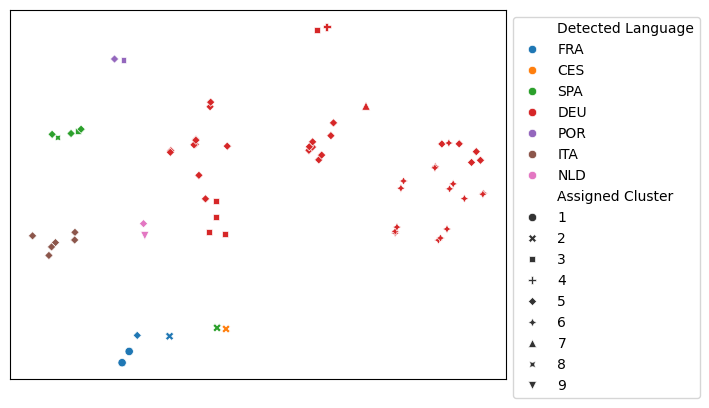
\includegraphics[width=0.5\textwidth]{data/images/tsne_plot_gpt4o.png}
        \label{fig:plot_gpt4o}
    }
    \end{subfigure}
    \vfill
    \begin{subfigure}[t-SNE plot of the baseline NewsStand cluster assignments.]{
        \centering
        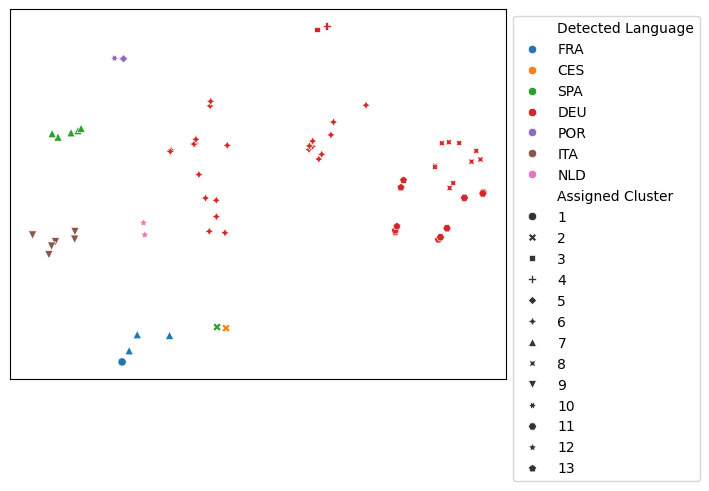
\includegraphics[width=0.5\textwidth]{data/images/tsne_plot_newsstand.png}
        \label{fig:plot_newsstand}
    }
    \end{subfigure}
    \caption{\textbf{t-SNE plots of NewsStandMULTI articles by language and cluster label for baseline cluster assignment and GPT-4o cluster assignment.}}\label{figure:tsne-plots} 
\end{figure}


% As we can see in the t-sne plot, the GPT embeddings, even when done without expressly stating the languages, form clear groups based on language.
% This suggests that while GPT is able to interface between several languages at once, it does not internalize meaning from them as being the same, embedding them differently depending on the language.
% Furthermore, when comparing the two plots, we can observe that clusterings for GPT tend to not fully be based off this embedding space, as can be seen in the Spanish section of the plot in the upper left, where 3 clusters are present rather than the 1 cluster present in the Newsstand data.




% The timeline plot reveals that gpt-4o does not account for language differences at all when prompted with the time.
% This leads to a poor clustering, in which the majority of articles are placed into the same cluster regardless of language or topic.
% In contrast, the NewsStand clustering algorithm groups the articles mostly via language, resulting in a much more even clustering.

% \begin{figure}[t]
%     \centering
%     \begin{subfigure}[t]{.45\textwidth}
%         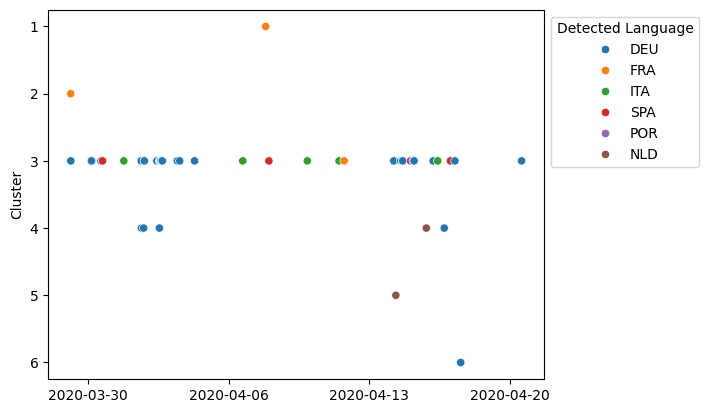
\includegraphics[width=0.5\textwidth]{data/images/timeline_plot_gpt4o.png}
%         \caption{\small Timeline plot of the gpt-4o clusterings. 6 data points omitted to better see detail in different times.} 
%         \label{fig:plot_length}
%     \end{subfigure}
%     \hfill
%     \begin{subfigure}[t]{.45\textwidth}
%         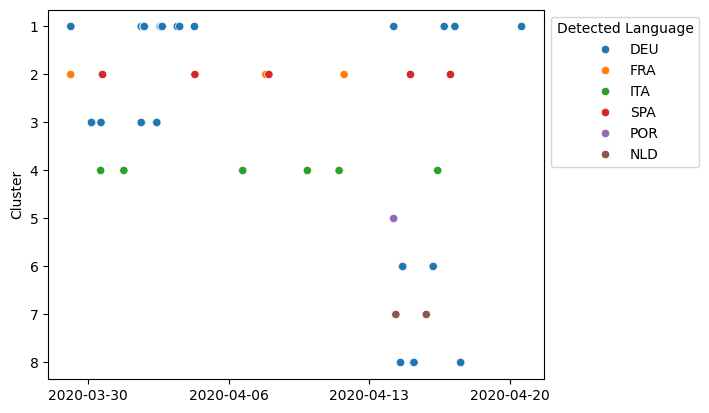
\includegraphics[width=0.5\textwidth]{data/images/timeline_plot_newsstand.png}
%         \caption{\small Timeline plot of the NewsStand clusterings. 6 data points omitted to better see detail in different times.} 
%         \label{fig:plot_beta}
%     \end{subfigure}
%     \caption{\textbf{Timeline plot of gpt-4o clusters vs NewsStand clusters}}\label{figure:time-plots} 
% \end{figure}


% \begin{figure}[t]
%     \centering
%     \begin{subfigure}[t]{.45\textwidth}
%         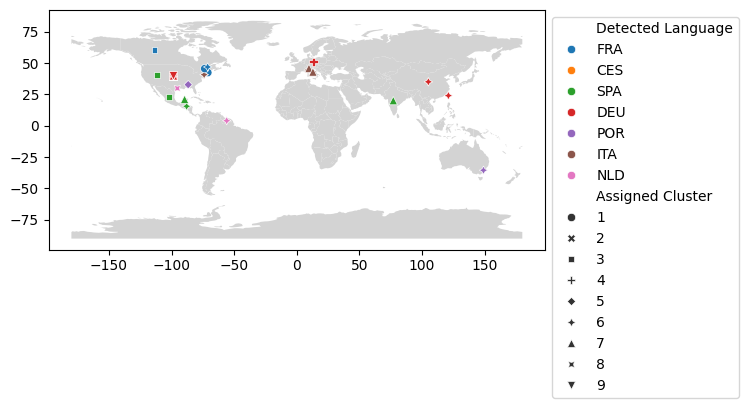
\includegraphics[width=0.5\textwidth]{data/images/map_plot_gpt4o.png}
%         \caption{\small Map plot of the gpt-4o clusterings.} 
%         \label{fig:plot_length}
%     \end{subfigure}
%     \hfill
%     \begin{subfigure}[t]{.45\textwidth}
%         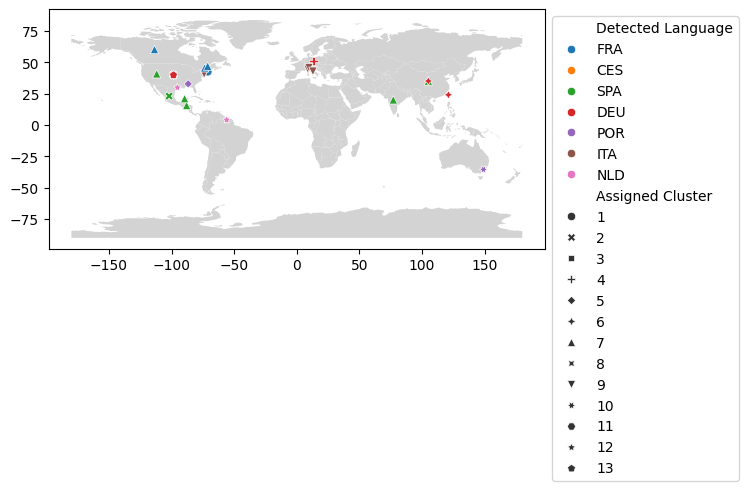
\includegraphics[width=0.5\textwidth]{data/images/map_plot_newsstand.png}
%         \caption{\small Map plot of the NewsStand clusterings.} 
%         \label{fig:plot_beta}
%     \end{subfigure}
%     \caption{\textbf{Timeline plot of gpt-4o clusters vs NewsStand clusters}}\label{figure:time-plots} 
% \end{figure}

Plotting the articles by time of publication in Figure \ref{figure:time-plots}, we compare the cluster assignments made by the baseline method and by GPT-4o.
In the baseline cluster assignment, clusters 3, 6, 7, and 8 are correlated with time, since the articles grouped in those clusters were all published within a few days of each other.
On the other hand, there were no clusters by GPT-4o that showed this same property.
Instead, the majority of the articles were grouped into one cluster, cluster 3, regardless of time of publication.
Most of those articles were written in German, indicating the LLM clustered based on language more than time of publication, which is contrary to the goal of cross-lingual clustering of news articles.


\subsubsection{Qualitative Analysis}

Qualitatively analyzing the clustering results produced by the LLMs, we further find that clusters typically correspond to the language of the text, rather than the text content.
We identified many clusters corresponding to entirely Italian, Spanish, French, or German articles.
Likewise, the keywords generated by the LLMs to maintain the cluster topics were in that same language.
On the other hand, when analyzing the clusters generated by the baseline method, articles in most clusters were mixed across different languages, but were tied by a common topic, often corresponding directly to a single news event.
We also observed a similar phenomenon to the single language setting, where the LLMs sometimes associated nonsensical keywords with some of the clusters, which often corresponded to instances where clusters contained unrelated documents.

% \subsection{Cross-Lingual Keyphrase Extraction}

% \nrscomment{report what percent of the keywords reported by the LLM are proper nouns vs. other POS types and compare to distributions given in original paper. Are they mostly proper nouns like the original paper suggests should be the main driver of cluster behavior?}


% \subsection{Cross-Lingual Cluster Correction}

% \nrscomment{qualitatively evaluate if changed points are in better or worse clusters. Analyze by language to see if some get moved correctly more than others.}

